\renewcommand\thechapter{\Roman{chapter}}
\chapter{Realization and Implementation}
\newpage
\addcontentsline{toc}{section}{Introduction}

\section*{Introduction}
In this chapter we will present the implementation and realization of our platform.\\We begin by presenting the application's architecture. Then we present the software and hardware environment along with the tools used. Afterwards, we will give an overview of the modules that are working in the platform to do the analysis and security measures implemented following earlier specifications.


\section{Application’s Architecture}
In this section we will introduce the architecture we followed for developing and deploying the platform.
\subsection{General Architecture}
For better usability, modifiability, stability, and security, we chose to follow a simple architecture that consists of a client and a server.\\With the server being centralized, the client server architecture, seen in Figure III.1, allows the application to manage resources common to all users, allow the use of the application without depending on the user's own computer specifications, which is an important factor considering the processing of E-evidence, and also presents more secure infrastructure since administrators can control consultants data access on server with relatively little effort, so the system can be upgraded simultaneously for all users in no time.\\With the user accessing through the client, which is any web browser, instructions are sent as HTTP requests to the server, then the server processes the data using pre-made scripts and send a reply.
\begin{figure}[H]
\centering
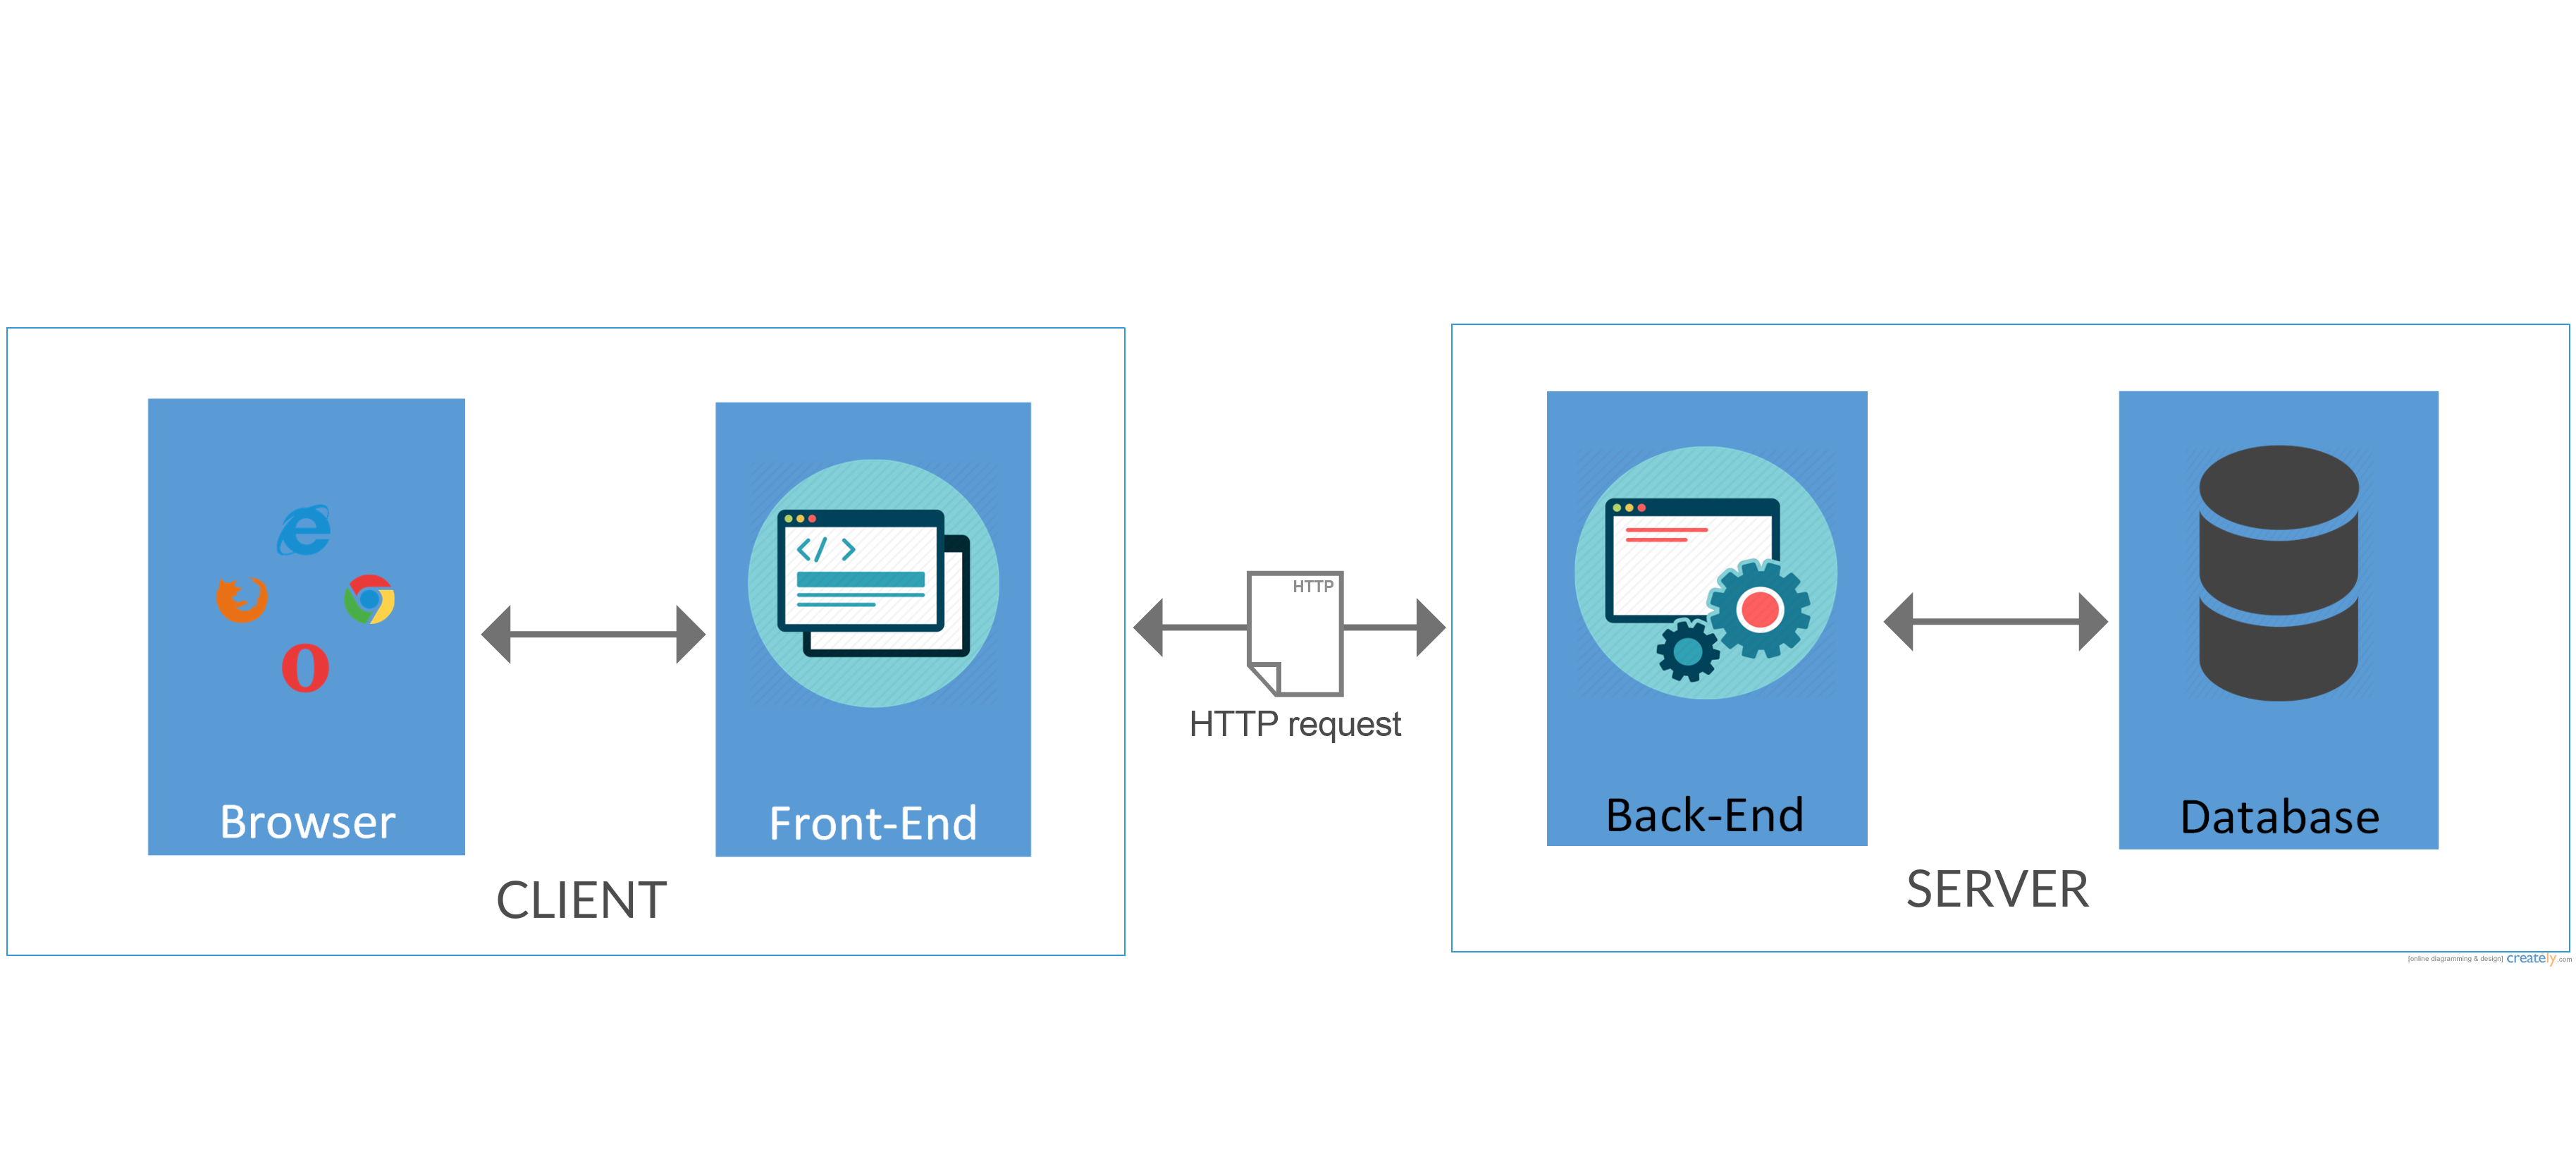
\includegraphics[width=1\columnwidth]{Figures/genarchitecture.png}
\caption{General architecture of the application}
\end{figure}

\subsection{Server and Back-End Architecture}
The application's back-end architecture uses Django views as controller and executor of instructions received from the client. The view does the back-end work related to the interface by accessing the database for requesting data to be shown on the platform, or sending data inserted by the users.\\As for the analysis, it is done by pre-made python scripts for each forensic analysis type. Each type has it's own modules implemented and requested by a relative script which is requested by the view and connects to the database for accessing case data or saving analysis reports. The Figure III.2 presents an overview of the connections between the Back-End server components:
\begin{figure}[H]
\centering
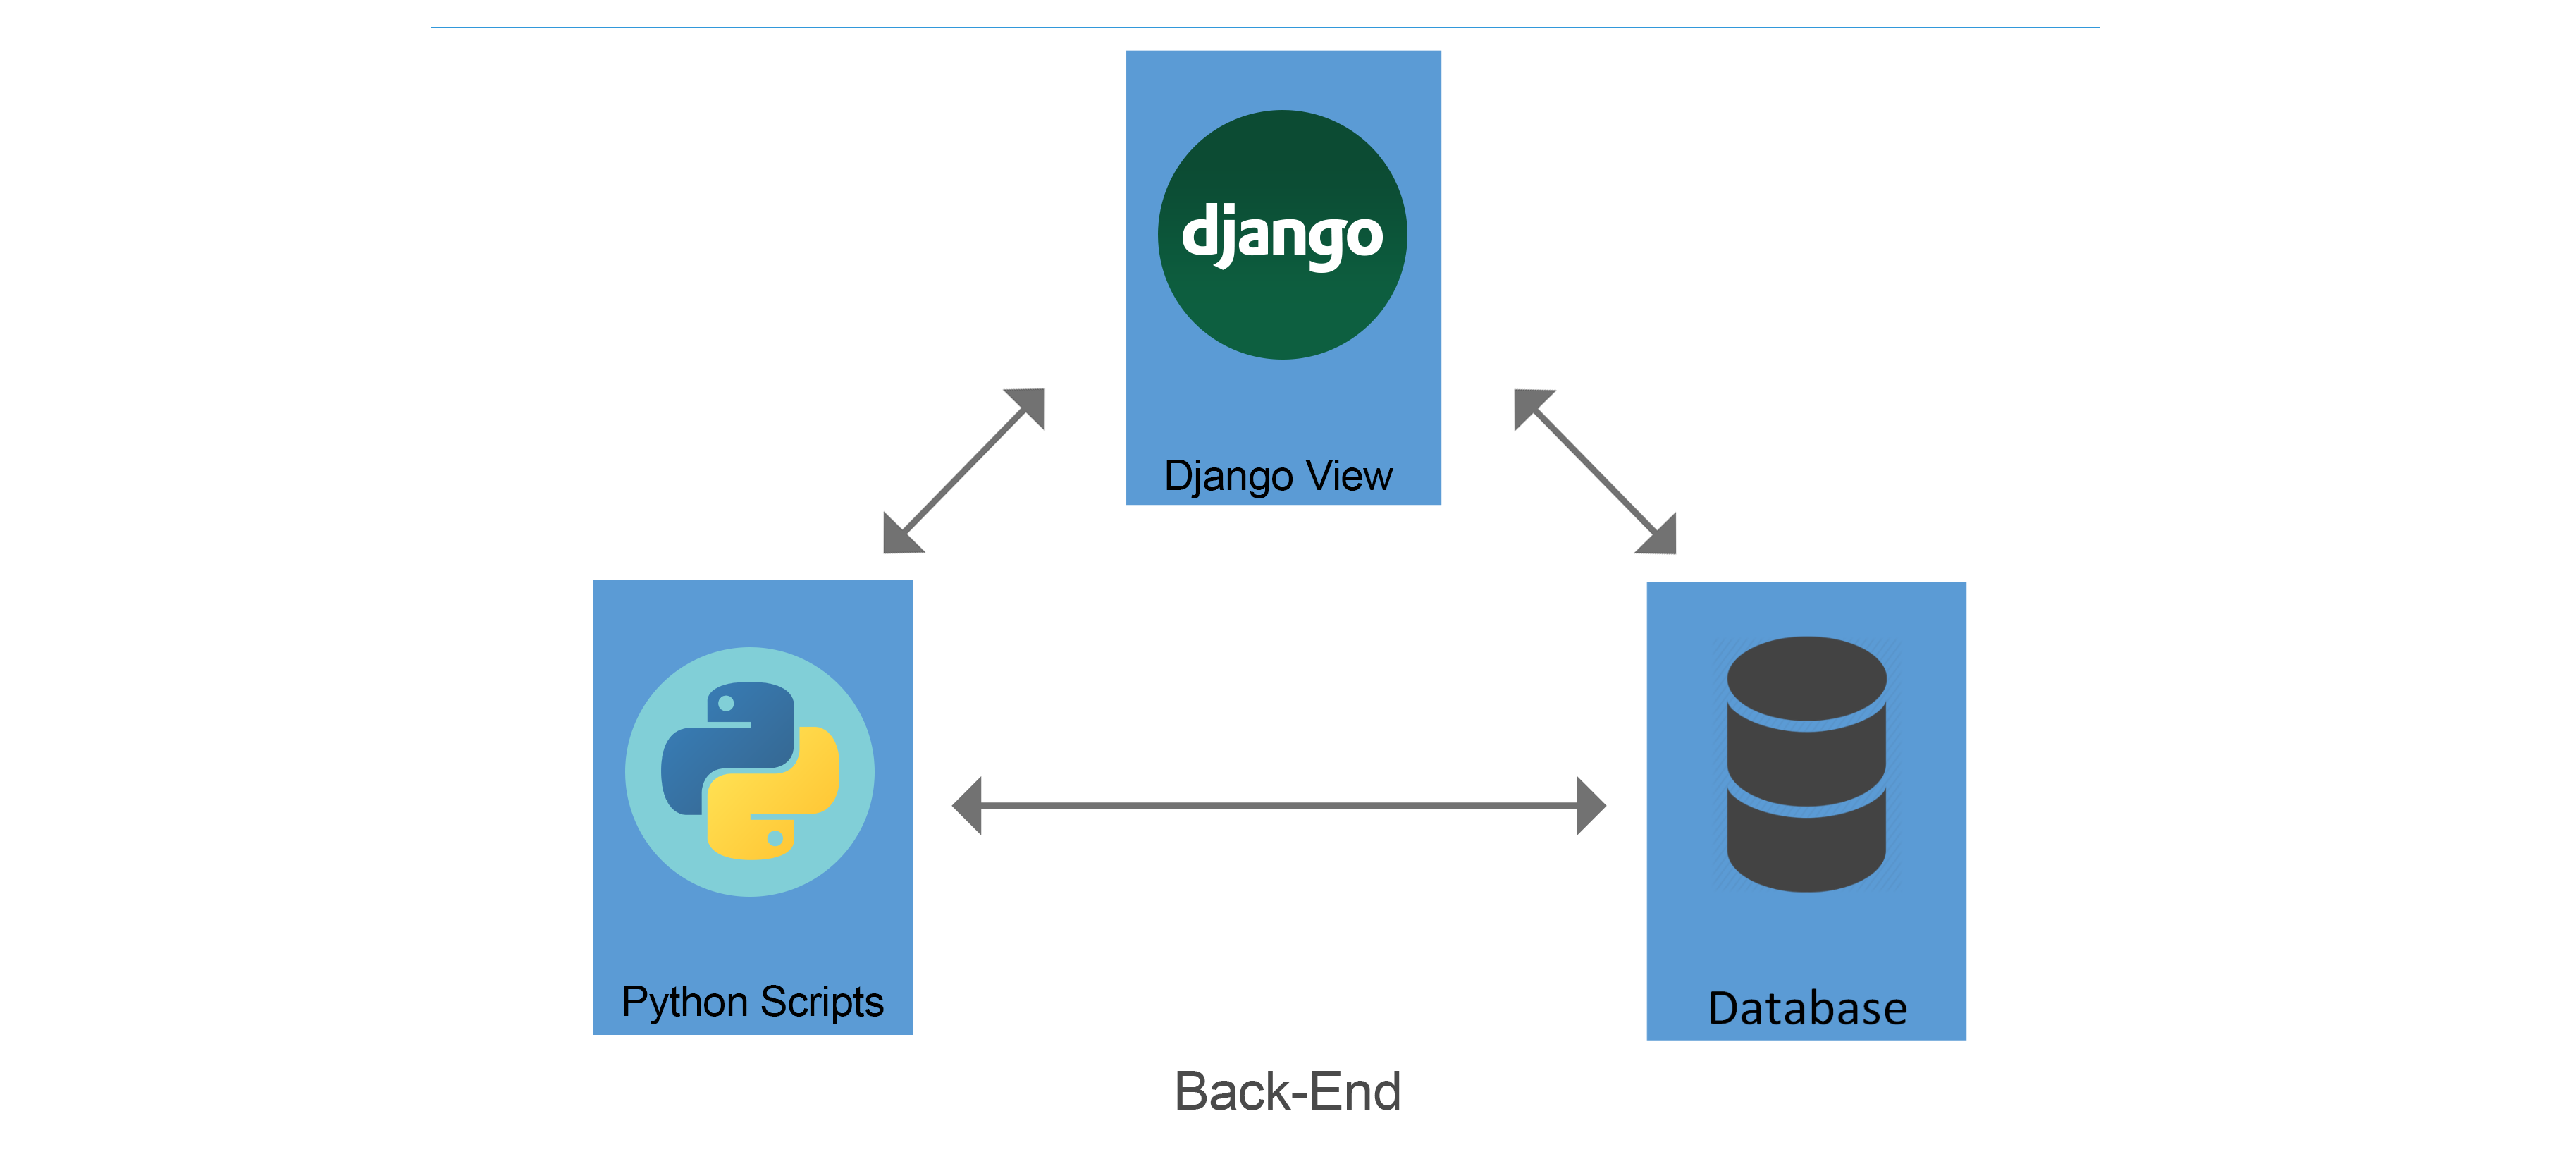
\includegraphics[width=1\columnwidth]{Figures/backarchitecture.png}
\caption{Back-End architecture}
\end{figure}
The application will Preserve the evidence, Identify it, Process it, Analyse and Interpret the analysis, and lastly Present the findings as clear as possible. The forensic analysis types that we included in the platform are the following:
\begin{itemize}
    \item Memory analysis
    \item Network analysis
    \item Disk analysis
\end{itemize}


\section{Software and hardware environment}
We will present the various technologies and tools that we have used and implemented over the platform.
\subsection{Hardware environment}
The process of analysing digital evidence such as memory and disk requires high-end specifications for rapidity and efficiency. So, during most of the project phases, we used a machine that had the specifications presented bellow.\\
\textbf{Laptop:}
\begin{itemize}
    \item \textbf{CPU:} Intel Core i7 6700HQ @ 2.60GHz
    \item \textbf{GPU:} NVIDIA GeForce GTX 960M 4GB
    \item \textbf{RAM:} 16GB SDRAM DDR3
    \item \textbf{Disk:} SSD 120GB / HDD 1TB
    \item \textbf{OS:} Parrot OS
\end{itemize}
For the testing phase, we used virtual machines to separate our production and testing environments. The VMs will not be included in the platform architecture since they were used to replicate a real use case.
\begin{itemize}
    \item \textbf{Hypervisor:} Virtualbox 6.0
    \item \textbf{Virtual machine 1:} 
        \begin{itemize}
            \item CPU: 4
            \item RAM: 4GB
            \item Disk: 80GB
            \item OS: Kali Linux 2019.1
        \end{itemize}
    \item \textbf{Virtual machine 2:} 
        \begin{itemize}
            \item CPU: 1
            \item RAM: 2GB
            \item Disk: 32GB
            \item OS: Windows 7 Pro 64bit
        \end{itemize}
\end{itemize}

\subsection{Software environment and technologies}
In this section, we are going to present the tools and software we used in the development of the platform, and justify each of these choices.
\subsubsection{IDE}
Using and IDE provides comprehensive facilities for software development like integrated tools and add-ons that make the development process clearer and more efficient. Sublime text, Visual Studio, and PyCharm are some of the best IDEs favored all over the world. Our choice was PyCharm\cite{pycharm} which is dedicated for Python, available in both paid and free version while introducing amazing advantages and work on Windows, Mac OS X, and Linux platforms. This IDE supports Python development directly and is therefore well suited for Django developing. The paid version also supports Django development out of the box. It also contains powerful tools for debugging, an integrated terminal, and also an integrated python interactive shell. This makes it quite easy to manage a project with a big infrastructure that also requires moving through lots of windows.

\subsubsection{Hypervisor}
A hypervisor allows the creation of multiple virtual machines on a single computer. This gives us an oppurtunity to create a testing environment that is easy to use, reset, and maintain. In comparison to VMware ESXi and Hyper-V, VirtualBox\cite{virtualbox} was the best solution to choose between them. It allows creating virtual machines, each with an operating system, on a running Machine inside a host operating system, making it a type 2 hypervisor. The architecture used by virtualbox is more useful and appropriate in our case. We also don't want to sacrifice our host OS, and are using the virtual machines for creating test cases. Another advantage is that virtualbox uses easier and more compatible file types for the snapshots and disk storage, which we will use for testing our platform.

\subsubsection{Front-end framework}
Django is a high-level Python open-source web application development framework that provides a clean and pragmatic design to database-driven websites. It has a good set of libraries and underscores effectiveness, allows less need for coding and reusability, and also various secure measures. It is also based on the Model-Template-View (MTV) architecture which is close to the MVC architecture. It also comes with a ready administration interface that allows administrators to easily add, edit, and remove users, models and consult recent changes by users in the website's database. Looking for long-term support for the platform, Django is also perfect for supporting Python3 since Python2 is to be out of support starting 2020.


\subsubsection{Back-end}
For the back-end, we need a scripting language that is well supported in information security. There are multiple choices including Ruby, Python, and Go. Our choice falls on Python for various reasons including preference, the tools we will implement also use it, and the libraries it provides prove very useful for our platform.
Python is an object-oriented, high-level programming language built for general purpose programming with integrated dynamic semantics for scripting, web and app development, and recently popular in data science. The large libraries and community support for Python keeps it one of the best, easiest, and favorite programming languages. Python is well suited for usage in the cyber security field since it has a clean, dynamic and logical syntax code and modular design. Also the need for programming in cyber security is high, so python being an interpreted scripting language with an immersive library, not to mention it's growth to the top lists, makes it the obvious choice. One of the libraries we used to connect the database to the front-end was the following:
\begin{itemize}
    \item Djongo
    Django doesn't usually come supported to MongoDB since the latter is a NoSQL database. Using Djongo we can make it possible to use Django with MongoDB without changing the Django ORM (Object-Relational Mapper). Djongo serves as a SQL to MongoDB query compiler. It basically translates a SQL query into a MongoDB query document.
\end{itemize}

\subsubsection{Database management}
The design for non-SQL databases is relatively simple, speed tolerant, and more flexible. MongoDB is a document-oriented database classified as a NoSQL database, meaning it doesn't follow the tabular relations for storage and retrieval of data like other SQL or relational databases. MongoDB uses JSON-like documents, which is one of it's powerful traits since JSON is replacing XML as a standard data interchanging language. More and more scripts, tools, and APIs now output results as JSON data, which makes it perfect for us to use it as our back-end database.


\subsubsection{Open-source used tools}
We implemented well-known and used open source tools in the platform which helps us get accurate results and edit the code per our needs. The reason for choosing these tools is because they've proven their usefulness regarding the modules we are implementing. We will now list the tools we used in our solution:
\begin{enumerate}
    \item \textsc{Volatility }
         is an open-source forensics framework for incident response and malware analysis on memory analysis implemented in python. It supports analysing memory of multiple operating systems like Linux, Windows, Mac, and Android, and can analyse different volatile memory samples such as raw dumps, crash dumps, and virtual machines memory dumps.
    \item \textsc{CapTipper }
         is a python tool providing a way to analyze, explore and revive HTTP malicious traffic. It mainly recreates a web server like the one in the traffic from the provided pcap file and allows inspection. The tool also contains an interactive console for deeper analysis of traffic and trasfered objects.
    \item \textsc{Tcpxract }
         is a tool written in C language for carving files from pcap files by analyzing data streams. It tries to identify and extract the files in the sessions using file file signatures and started at first using the same technique as Foremost for recovery.
    \item \textsc{Foremost }
         is a tool used for data carving from files, and was originally created for law enforcement uses. It searches for files using built-in types signatures, headers, and data structure. Foremost work mainly with disk images created by dd, Encase, and other tools. It can recover deleted files from a drive that hasn't been override by zeros.
\end{enumerate}


\section{Application’s Implementation}
This section contains the technical implementation of the platform and the modules in each forensic analysis type. Then we will introduce some of the implemented security measures. 
\subsection{Memory Forensics}
For the memory forensics, the script is provided with a case object to analyse. The script for this subsystem then gets the evidence file provided and starting running various modules that consist mostly of Volatility plugins and in which some are custom made.\\
The volatility plugins included are saved in the appropriate directory relative to the tool which is included with our platform by default. In the case of these plugins, we'll loop through a pre-made list, which takes place in a settings file included in the script, while selecting a certain extraction file type and location for each one as Figure III.3 shows:
\begin{figure}[H]
\centering
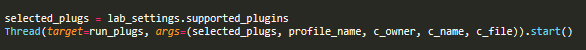
\includegraphics[width=1\columnwidth]{Figures/1_.png}
\caption{Volatility plugins call}
\end{figure}
The Figure III.4 shows the different arguments passed to Volatility when calling certain plugins due to their unique requirements.
\begin{figure}[H]
\centering
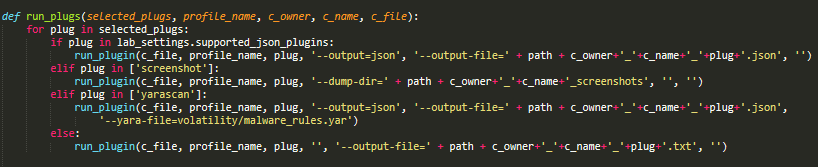
\includegraphics[width=1\columnwidth]{Figures/2_.png}
\caption{Looping through and running Volatility plugins}
\end{figure}
We will now talk more about the modules individually. The modules as we said include and are not limited to Volatility plugins, customs modules, and APIs. We will present in the following subsections what each of the modules is doing.

\subsubsection{Keylogger Static Detection}
Keyloggers can be detected and identified as malicious applications for recording the user's activity such as keystrokes, screenshots, and network data. Keyloggers will need certain permissions that are known to be found on Spyware so it will most likely be detected in a dynamic analysis, but since a keylogger has high impact, we chose to develop a module which detects known Keyloggers for easier interaction. We will provide a list of well known keylogger process names in this case, and we'll be back for more advanced malicious application detection in later modules. We can see the combination between the process list and the keylogger list in Figure III.5 bellow.
\begin{figure}[H]
\centering
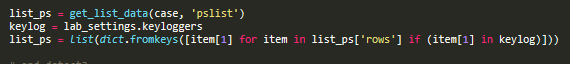
\includegraphics[width=0.8\columnwidth]{Figures/keyloggers.png}
\caption{Keylogger static detection code}
\end{figure}

\subsubsection{Malicious IP detection}
Based on the list of connections that we can extract using the Volatility 'netscan' plugin, we will remove local IP addresses and search the remaining ones on the web for previous violations or malicious traffic. This process only supports IPv4 for now.\\
For this module we use the API provided by AbuseIPDB\cite{abuseip} which will give us the number of reports registered against a certain IP and based on that, it calculates a trust level. We will be saving and outputting IPs with a relatively low trust level. The Figure III.6 explains how we loop through the IPs extracted from another module and scan each one of them as desribed above.
\begin{figure}[H]
\centering
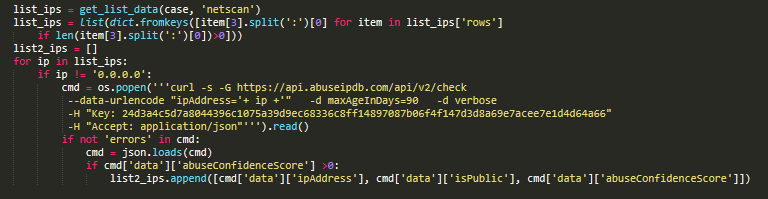
\includegraphics[width=0.8\columnwidth]{Figures/ips.png}
\caption{Malicious IP detection}
\end{figure}

\subsubsection{Process Extraction}
\begin{enumerate}[label=(\alph*)]
    \item \textbf{Process List}\\
    For listing the running processes on the system, we will use the 'pslist' plugin. We call volatility and simply ask for a process list. This will output the process name, pid, ppid, launch time, and other details.\\
    The module walk through doubly-linked list pointed to by PsActiveProcessHead to extract these process information as we see in Figure III.7, the plugin looks for all the processes.\\
    \begin{figure}[H]
    \centering
    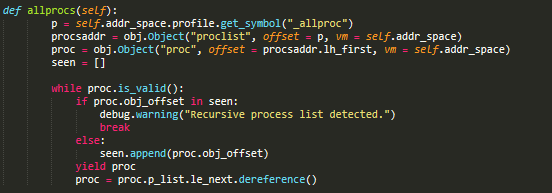
\includegraphics[width=0.8\columnwidth]{Figures/pslist.png}
    \caption{Process list core extraction from memory}
    \end{figure}
    After listing all processes, we can extract the process executable file from memory by supplying the offset to the 'procdump' plugin. And of course this is done automatically. Figure III.8 contains the code we wrote to combine the previous extracted info, primarily the process pid, with the 'procdump' plugin to extract the executable.
    \begin{figure}[H]
    \centering
    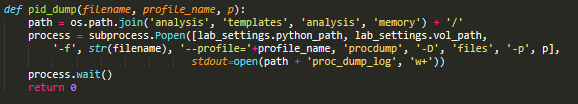
\includegraphics[width=0.8\columnwidth]{Figures/psdump.png}
    \caption{Process dumping function}
    \end{figure}
    \item \textbf{Process Tree}\\
    The process list extracted by the previous module is more accurate than this one, but also not enough for following the root of a process. For that reason comes a need to scan the process explorer to output a tree representing the processes each under it's parent.\\
    This module uses Volatility's 'pstree' plugin, which simulates the execution of the command called with the same name under Linux systems. The latter being a visual representation of the process list while the root of the tree is mainly init. The process for extraction starts by finding the root then the next node and the nodes following it. The next figure, Figure III.9, shows the first step of the process.
    \begin{figure}[H]
    \centering
    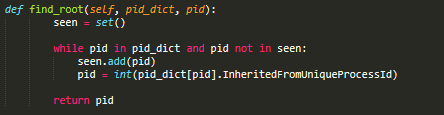
\includegraphics[width=0.8\columnwidth]{Figures/pstree.png}
    \caption{Process tree root location}
    \end{figure}
\end{enumerate}

\subsubsection{Auto-run Programs Scan}
This module uses a volatility custom-made by Tomchop\cite{tomchop} and it allows finding Auto-Start Extensibility Points or Persistence Points which is a recurring task of any investigation to locate potential software that is doubted as malware.\\
Modern Malware and especially Trojans that run in memory need to be started every time a computer is powered-up, that is why we need to analyse autorun programs.\\
This module basically automates the tasks you would need to identify where malware or a certain process is persisting from. Depending on the system, after all the auto-start locations are found, they are matched with running processes to finally output a list. The full code of the plugin can be found on it's repository\cite{autorun_repo}. The Figure III.10 contains a portion of the locations included in the search:
\begin{figure}[H]
\centering
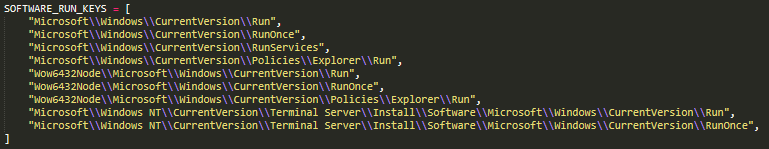
\includegraphics[width=0.8\columnwidth]{Figures/autoruns.png}
\caption{List from the lists of location to search}
\end{figure}

\subsubsection{Network Scan}
To get a list of network connections made on a computer out of a memory dump, we will use Volatility's 'netscan' plugin. This plugin was introduced around 2011 and gives an overview of the active and inactive connections on a computer.\\
Without getting into physical memory or the plugin's details, this module find TCP/UDP endpoints, which establishes connections, and TCP/UDP listeners, which listens for connection on a certain port. It also has the ability to distinguish and regroup connection based on the IP version used (IPv4 / IPv6) and local/remote IPs.\\
The plugin is good to give us an overview to establish a timeline based on other data that it extracts like the time when the socket was bound or the connection was established, and it's current state.
%image

\subsubsection{Physical Files Scan}
Using the 'filescan' plugin from Volatility, we can scan the memory dump for file objects, which will find a file by the hooks and pointers defined when processes use it. We can then extract these files from memory or follow the pointers to the processes and go deep into injected DLLs.\\
Technically talking, the process is used for locating kernel object allocations using pool tag scanning. The module shows permissions affected to the files, physical offset, number of pointers and handles to the file object.\\
We then try to extract the file, on demand, using the 'dumpfiles' plugin, as seen in Figure III.11. This can be done by using the already-found offset of the object. Some files can't be extracted for various reasons, one of them being that the file is just a Symbolic link to another file meaning it's not the physical file having the real contents.
\begin{figure}[H]
\centering
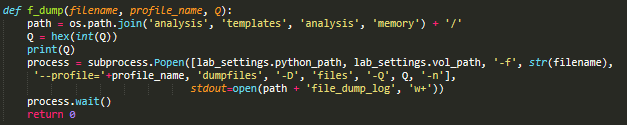
\includegraphics[width=0.8\columnwidth]{Figures/filedump.png}
\caption{File dumping function}
\end{figure}

\subsubsection{Browser Data Extraction}
Extracting Data from web browsers is important for following the user's footsteps and understanding it. The data can be his browse history, download history, cookies, and more. Since most of these data can be found in disk analysis and is not only relevant to memory, we'll be extracting only browsing history.\\
Each browser stores the user's data in it's specific way. This module will allow us to go through top used web browsers on windows to extract it's history from memory.
\begin{enumerate}[label=(\alph*)]
    \item \textbf{Internet Explorer history}\\
    For Internet Explorer the plugin builds a list of tags based on the selected command-line options and associate the tags with our \_URL\_RECORD and \_REDR\_RECORD structures.
    \item \textbf{Google Chrome history}\\
    Google Chrome saves all the data in an SQLite database encrypted using the user's password, and since we're working on the memory itself, we get unencrypted data. Then, the module extracts records from the Chrome urls table in the database file. The plugin is named 'chromehistory' and is created by Superponible\cite{superponible}.
    \item \textbf{Mozilla Firefox history}\\
    Firefox, like Chrome uses it's own database and makes a profile folder in a known location. The 'firefoxhistory' plugin, also created by Superponible, extracts records from the Firefox moz\_places table in the places.sqlite SQLite database file.
\end{enumerate}
%image for iehistory only

\subsubsection{Command Line Detection}
\begin{enumerate}[label=(\alph*)]
    \item \textbf{Command history}\\
    The 'cmdscan' plugin from Volatility is used here to search the memory of csrss.exe and conhost.exe on relative Windows versions for commands that attackers or users may have entered through a console. This module finds structures known as COMMAND\_HISTORY by trying to look for the known constant value MaxHistory (usually set to 50) and then applying sanity checks.
    %image
    \item \textbf{Process commands}\\
    This module uses the 'cmdline' plugin to detect process parameters and arguments and extract the complete command line used to start the process from background CLI in the first place. The plugin generates the command line from the data acquired by the DLL files.
    %image
\end{enumerate}


\subsubsection{Graphical User Interface Scan}
This module draws frames of the GUI from the memory based on opened windows. It is far from a real screenshot but shows outlines, windows names, and possibly underlying windows. It basically enumerates windows for each desktop in their Z-Order. An example of the output pictures is included in Figure III.12:
\begin{figure}[H]
\centering
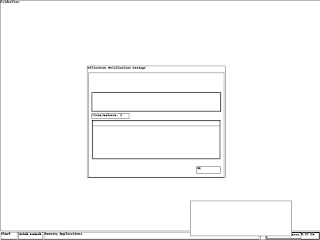
\includegraphics[width=0.8\columnwidth]{Figures/vol_screen.png}
\caption{Memory screenshot output example}
\end{figure}

\subsubsection{Malware Analysis}
For detecting malware, we use some simple techniques that try to search for malicious-known data inside a process to identify it as a malware, or locate injected DLLs, or have certain permissions like network access or system files write.
\begin{enumerate}[label=(\alph*)]
    \item \textbf{Malfind}\\
     Based on characteristics such as VAD tag (virtual address descriptor) and page permissions, The 'malfind' plugin tries to locate injected shellcode or DLLs that basic methods can't find. An example of injection that it can't detect are the ones initiated using CreateRemoteThread.
    \item \textbf{YARA scan}\\
     The purpose of YARA is to identify and classify malware samples. YARA rules provide a way to create descriptions for malware families based on textual or binary patterns that the determine the logic behind the malware. This makes YARA as the main way that could detect malware without reversing an executable.\\
     Using these rules, the 'yarascan' plugin, provided with a custom file containing various rules of malware and malicious applications, can detect a malicious process when comparing it's data and behaviour to a certain rule.
     \begin{figure}[H]
     \centering
     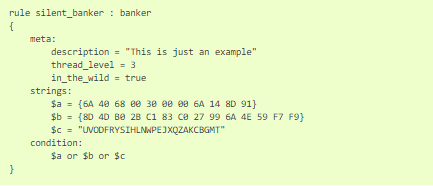
\includegraphics[width=0.8\columnwidth]{Figures/yara.png}
     \caption{YARA rule description example}
     \end{figure}
     The rule, in Figure III.13 above, is telling YARA that any file containing one of the three strings must be reported as silent\_banker. This is just a simple example, more complex and powerful rules can be created by using wild-cards, case-insensitive strings, regular expressions, special operators and many other features that you’ll find explained in this documentation\cite{yara_doc}.
\end{enumerate}


\subsubsection{User Password Extraction}
\begin{enumerate}[label=(\alph*)]
    \item \textbf{Hashdump}\\
    The 'hashdump' plugin accesses the SAM and SYSTEM hives on Windows registry and outputs cached user credentials which can possibly be cracked later.
    \item \textbf{Mimikatz}\\
    Mimikatz was first a tool that extracts plain text passwords from Windows. The module introduced as a Volatility plugin works the same as in a live machine by analysing the LSASS process, finds the encryption keys and IV (initialization vector) and decrypts the hashed passwords in the LSA Secrets registry. The plugin contains decryption functions relative to most windows versions. We can see the function relative to the 64 bit version of Windows 7 in Figure III.14.
    \begin{figure}[H]
    \centering
    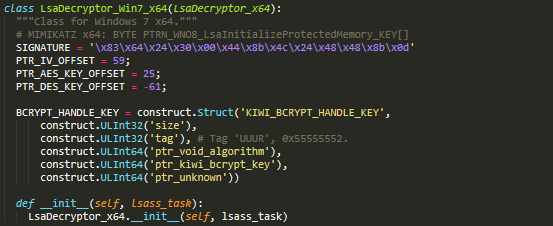
\includegraphics[width=0.8\columnwidth]{Figures/mimikatz.png}
    \caption{Mimikatz plugin - LSADecryptor for Win7 64bit}
    \end{figure}
\end{enumerate}


\subsection{Network Forensics}
\subsubsection{HTTP malicious traffic detection}
Drive-by attacks are when a victim is redirected through multiple websites until he lands on a malicious server that hosts an exploit kit. The exploit kit scans the victim's computer and installs or executes a malware, such as a flash script, javascript, or an executable on the computer to get access. To detect these traffics we used CapTipper\cite{captipper} to analyse our network traffic. The tool launches a web server and replay the pcap file while intercepting the traffic. We then get the output of the first stage analysis which is a summary since the tool also offers an advanced interpreter. We run the script from the directory saved in the settings and save the output to a file to be processed later, as shown on Figure III.15 bellow.
\begin{figure}[H]
\centering
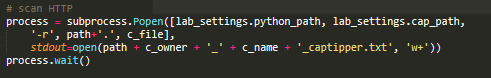
\includegraphics[width=0.8\columnwidth]{Figures/http.png}
\caption{Calling CapTipper from settings}
\end{figure}

\subsubsection{File carving}
Detecting and extracting communicated files on the network is important even if our automated analysis doesn't detect it is malicious at first. So using Tcpxtract, we supply a pcap file and try to carve out files using the list of file signatures that we know. As shown in Figure III.16, we simply provide the file as an argument to the tool.
\begin{figure}[H]
\centering
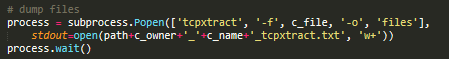
\includegraphics[width=0.8\columnwidth]{Figures/tcpx.png}
\caption{File carving using tcpxtract}
\end{figure}

\subsection{Disk Forensics}
\subsubsection*{File extraction}
Files can be deleted from a drive but unless the space was rewritten to zeros, we can recover the files using Binwalk and Foremost file carving technique that depends on file signatures, footers, and structures. Shown in Figure III.17 is the usage of binwalk in our module. The tool simply needs a disk image and will automatically try to find out files and save them in an output folder.
\begin{figure}[H]
\centering
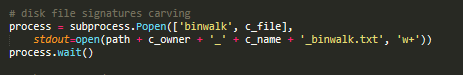
\includegraphics[width=0.8\columnwidth]{Figures/disk.png}
\caption{File extraction using Binwalk}
\end{figure}

\subsection{Secure measures}
\subsubsection{Encrypted traffic}
Normally, data sent between browsers and web servers is in plain text, leaving users vulnerable to eavesdropping. If a malicious party intercepts the data that's being transferred between a client and a web server, they can see and use that information and the user would be vulnerable to MITM attacks.\\
SSL enables secure exchange of information between browsers and the web server, that's why we used an SSL certificate to secure the traffic using HTTPS. Figure III.18 presents the details of our used certificate in the web server.
\begin{figure}[H]
\centering
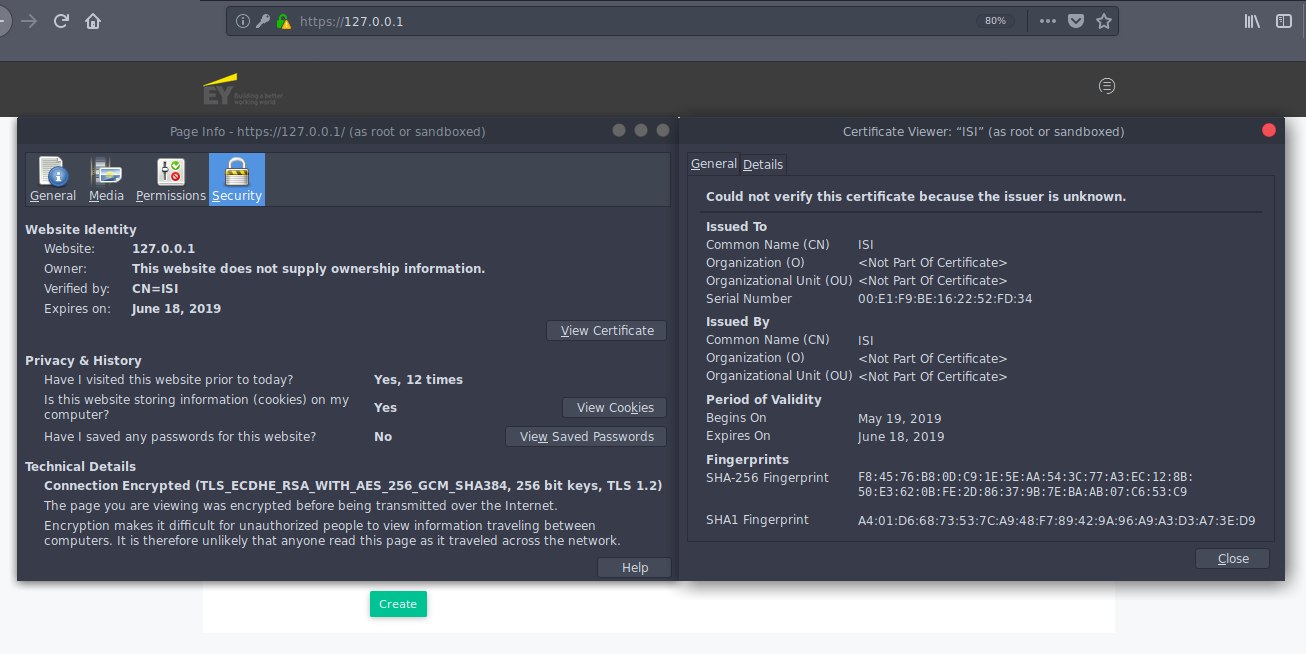
\includegraphics[width=0.8\columnwidth]{Figures/ssl.png}
\caption{SSL certificate details}
\end{figure}
\subsubsection{Authentication}
Django provides a flexible password storage system and uses PBKDF2 with sha256 by default \cite{dj_auth}. The password is stored in the following format:
\begin{verbatim}
    <algorithm>$<iterations>$<salt>$<hash>
\end{verbatim}
The code responsible for generating the password is represented in Figure III.19.
\begin{figure}[H]
\centering
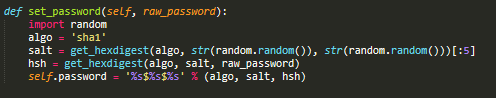
\includegraphics[width=0.8\columnwidth]{Figures/password_storage.png}
\caption{Django password storing mechanism}
\end{figure}

\subsubsection{Cross site request forgery protection}
CSRF attacks allow a malicious user to execute actions using another user's session without the latter’s knowledge or consent.\\
For this reason Django provides us with a built-in tag \{\%csrf\_token\%\} to be used inside action forms on the template side. In Figure III.20, we show a portion of the login page's template, where we used the provided tag inside the authentication form.
\begin{figure}[H]
\centering
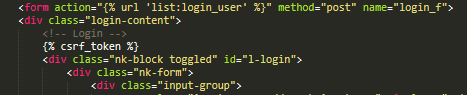
\includegraphics[width=0.8\columnwidth]{Figures/csrf.png}
\caption{CSRF tag in login form}
\end{figure}

\subsubsection{Input filtration for RCE protection}
Using the uploaded evidence files in multiple commands explicitly exposes the back-end server to Remote Code Execution (RCE). This requires either trusting the user's input or filtering it to remove any possible bypass method.\\
As a first step we renamed the uploaded file to something that isn't exposed to the user using the code in Figure III.21. And that was achieved by not exposing the uploads directory to the public too.
\begin{figure}[H]
\centering
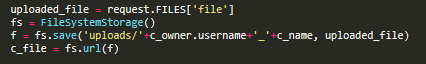
\includegraphics[width=0.8\columnwidth]{Figures/filename.png}
\caption{File naming}
\end{figure}
The second step was to filter the name of the case to avoid a bypass since it's used in the file name and other locations. The filter shown on the code in Figure III.22, is custom-made following various payloads on remote code execution seen on a research\cite{payloadsallthings}.
\begin{figure}[H]
\centering
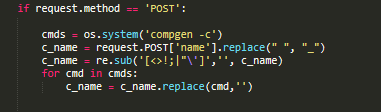
\includegraphics[width=0.8\columnwidth]{Figures/filter.png}
\caption{Case name filtering code}
\end{figure}




\section*{Conclusion}
\addcontentsline{toc}{section}{Conclusion}

Throughout this chapter, we introduced the general architecture of the platform including the front-end and back-end. We then described the environment by specifying the hardware and software used. Finally, we presented our core analysis modules technically, and also the security implementation in place.\\
In the next chapter, we are going to test our platform against a real case scenario while highlighting some of the modules.